% Provenance (never printed): see sources/outline_sources.md (Year 3:
% facies analysis, depositional models, Walther's law, well logs). Brief:
% sources/book5/BRIEFS.md, ch. 17. Curves from figdata/bachelor-3/well_logs.py
% (unit tops from figdata/shared/region.py). Exercise and problem values in
% the Book 5 scratch calculator calc/ch17.py. The well Varden-2, its logs and
% the channel architecture of its sandstone are invented.
\chapter{Modèles de faciès}\label{ch:b3:facies-models}

Une carotte prélevée dans un puits d'un kilomètre de profondeur~: un mètre de sable grossier
à stratification oblique reposant sur une base nette, passant vers le haut à des silts
marqués par des traces de racines, puis de nouveau du sable sur une autre base nette. Le
géologue y lit une rivière qui a divagué sur sa plaine, alors qu'aucun cours d'eau ne coule
plus à cet endroit. Cette lecture repose sur deux outils~: un ensemble de modèles, chacun
étant une synthèse de nombreux exemples actuels et anciens d'un même environnement, et une loi
qui transforme une succession verticale de couches en une carte des environnements voisins.

\begin{recall}
Les faciès sédimentaires, les milieux de dépôt, les formes de fond, la stratification oblique,
les deltas des trois types, les courants de turbidité, les turbidites et les bancs granoclassés
sont traités dans le volume de première année, au chapitre consacré aux sédiments détritiques
et à leurs milieux~; l'usine à carbonates, les récifs et les plates-formes carbonatées, dans le
chapitre consacré aux sédiments carbonatés, siliceux et évaporitiques~; le log de sondage
et la corrélation des logs, dans le chapitre consacré aux coupes. La porosité et la perméabilité
figurent dans les manuels du secondaire. Les \omterm{def:b3:sequence-stratigraphy:parasequence}{paraséquences}, les \omterm{def:b3:sequence-stratigraphy:parasequence}{surfaces d'inondation} et les
\omterm{def:b3:sequence-stratigraphy:tract}{cortèges sédimentaires} sont au chapitre~\ref{ch:b3:sequence-stratigraphy}. Les vagues en eau
profonde, dont le mouvement s'atténue avec la profondeur, sont traitées dans les volumes de physique.
\end{recall}

\section{Faciès, successions et loi de Walther}\label{sec:b3:facies-models:walther}

Un faciès sédimentaire se décrit à partir de ce que l'on voit dans une carotte ou sur une
falaise~: taille des grains, classement, structures, fossiles, couleur. Un faciès isolé est
rarement diagnostique~: du sable à stratification oblique se forme dans les rivières, sur les
plages, dans les chenaux de marée et dans les déserts. Ce qui identifie un milieu, ce sont les
faciès qui lui sont associés et l'ordre dans lequel ces faciès se succèdent.

\begin{definition}[Association de faciès et succession de faciès]\label{def:b3:facies-models:association}
Une \emph{association de faciès}\index{association de faciès} est un groupe de faciès
qui apparaissent ensemble et se sont déposés dans un même milieu, comme des sables de chenal,
des silts de levée et des boues de plaine d'inondation avec racines. Une \emph{succession de
faciès}\index{succession de faciès} est une suite verticale de faciès dans laquelle une
propriété évolue progressivement vers le haut~; dans une \emph{succession
granodécroissante}\index{succession granodécroissante}, la taille des grains diminue vers le haut,
tandis que dans une \emph{succession granocroissante}\index{succession granocroissante}
elle augmente.
\end{definition}

\begin{definition}[Modèle de faciès]\label{def:b3:facies-models:model}
Un \emph{modèle de faciès}\index{modèle de faciès} est une synthèse générale
d'un milieu de dépôt, établie à partir de nombreux exemples actuels et anciens~: les faciès
qu'il produit, leur géométrie, leurs relations latérales et les successions qu'ils forment.
Il sert de référence pour comparer un nouvel exemple, de guide pour les observations
ultérieures, de prédicteur dans des situations nouvelles et de base
pour interpréter le milieu.
\end{definition}

La liaison entre le latéral et le vertical repose sur une loi. Des milieux voisins se trouvent
côte à côte à un instant donné~: la plage à côté de l'\omterm{def:b3:facies-models:shoreface}{avant-côte}, l'\omterm{def:b3:facies-models:shoreface}{avant-côte} à côté de la
boue de plateau externe. Lorsque le rivage se déplace, chaque milieu vient se superposer
à son voisin.

\begin{theorem}[Loi de Walther]\label{thm:b3:facies-models:walther}
Dans une succession concordante, sans rupture significative de sédimentation ni surface
d'érosion, les faciès qui se superposent directement se sont déposés dans des milieux qui
étaient côte à côte à l'époque.
\end{theorem}

\begin{proof}
Considérons des ceintures de milieux, chacune étant une bande parallèle au rivage, qui
migrent ensemble à travers le bassin pendant que le socle s'affaisse ou que le niveau marin
monte. En un point fixe, les ceintures passent l'une après l'autre, dans l'ordre où elles
se trouvent côte à côte, et chacune laisse son dépôt au sommet de celui de la ceinture qui
l'a précédée. Si la sédimentation est continue, l'ordre vertical des dépôts est donc
l'ordre latéral des ceintures. Une lacune ou une surface d'érosion interrompt~:
le raisonnement~: les ceintures qui sont passées pendant l'intervalle n'ont rien laissé,
ou leurs dépôts ont été enlevés, et des faciès de milieux non adjacents
viennent alors au contact.
\end{proof}

\begin{omfigure}
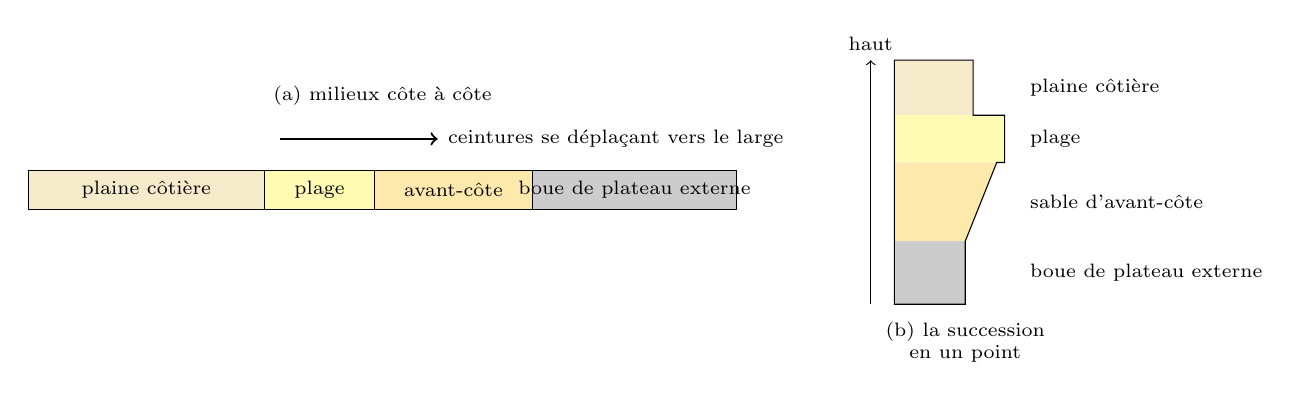
\begin{tikzpicture}[font=\scriptsize, x=1cm, y=1cm]
% environments side by side, with a shoreline that moves seaward
\fill[yellow!35!brown!25] (0,0) rectangle (3,0.5);
\fill[yellow!30] (3,0) rectangle (4.4,0.5);
\fill[yellow!50!orange!30] (4.4,0) rectangle (6.4,0.5);
\fill[black!20] (6.4,0) rectangle (9,0.5);
\draw (0,0) rectangle (9,0.5);
\foreach \x in {3,4.4,6.4} {\draw (\x,0) -- (\x,0.5);}
\node at (1.5,0.25) {plaine côtière};
\node at (3.7,0.25) {plage};
\node at (5.4,0.25) {avant-côte};
\node at (7.7,0.25) {boue de plateau externe};
\draw[->, thick] (3.2,0.9) -- (5.2,0.9) node[right] {ceintures se déplaçant vers le large};
\node[anchor=south] at (4.5,1.2) {(a) milieux côte à côte};
% vertical succession at a place
\begin{scope}[xshift=11cm, yshift=-1.2cm]
\fill[black!20] (0,0) rectangle (0.9,0.8);
\fill[yellow!50!orange!30] (0,0.8) -- (0.9,0.8) -- (1.3,1.8) -- (0,1.8) -- cycle;
\fill[yellow!30] (0,1.8) rectangle (1.4,2.4);
\fill[yellow!35!brown!25] (0,2.4) rectangle (1.0,3.1);
\draw (0,0) -- (0.9,0) -- (0.9,0.8) -- (1.3,1.8) -- (1.4,1.8) -- (1.4,2.4) -- (1.0,2.4) -- (1.0,3.1) -- (0,3.1) -- cycle;
\node[anchor=west] at (1.6,0.4) {boue de plateau externe};
\node[anchor=west] at (1.6,1.3) {sable d'avant-côte};
\node[anchor=west] at (1.6,2.1) {plage};
\node[anchor=west] at (1.6,2.75) {plaine côtière};
\draw[->] (-0.3,0) -- (-0.3,3.1) node[above] {haut};
\node[anchor=north, align=center] at (0.9,-0.1) {(b) la succession\\ en un point};
\end{scope}
\end{tikzpicture}

\par\smallskip{\small La loi de Walther. (a) Les milieux se succèdent côte à côte
le long d'un profil~; (b) à mesure que les ceintures migrent vers le large, un même lieu reçoit
d'abord la boue du large, puis le sable d'\omterm{def:b3:facies-models:shoreface}{avant-côte}, le sable de plage et les dépôts de plaine côtière~: une
\omterm{def:b3:facies-models:association}{succession granocroissante}, dans l'ordre des ceintures (la largeur dans le log
indique un grain plus grossier).}\label{fig:b3:facies-models:walther}
\end{omfigure}

La loi fonctionne dans les deux sens. Une régression empile les ceintures dans leur ordre
vers le large, de bas en haut, une transgression dans l'ordre inverse~; et une succession verticale lue dans une
carotte donne la carte des milieux voisins à l'époque considérée. Elle cesse de s'appliquer
précisément là où le chapitre~\ref{ch:b3:sequence-stratigraphy} place ses surfaces clés~:
au niveau d'une \omterm{def:b3:sequence-stratigraphy:sequence}{limite de séquence}, où l'exposition et l'érosion amènent du sable fluviatile
sur une boue de plate-forme, et au niveau d'une \omterm{def:b3:sequence-stratigraphy:parasequence}{surface d'inondation}, où la boue du large repose
directement sur la plaine côtière.

\section{Rivières}\label{sec:b3:facies-models:rivers}

\begin{definition}[Rivières en tresses et rivières à méandres]\label{def:b3:facies-models:rivers}
Une \emph{rivière en tresses}\index{rivière en tresses} s'écoule dans plusieurs chenaux peu profonds
qui se divisent et se rejoignent autour de barres, sur une plaine à forte pente, chargée abondamment en matériaux grossiers
et à débit variable. Une \emph{rivière à méandres}\index{rivière à méandres}
s'écoule dans un chenal unique et sinueux, sur une plaine plus douce, transportant davantage
de sédiments fins~; elle migre en érodant la rive externe de chaque courbe et
en déposant sur la rive interne. Le dépôt de la rive interne est une \emph{barre de
méandre}\index{barre de méandre}. L'\emph{avulsion}\index{avulsion} est
l'abandon d'un chenal pour un nouveau tracé à travers la plaine d'inondation, généralement après qu'une crue
a rompu une digue naturelle.
\end{definition}

Une \omterm{def:b3:facies-models:rivers}{barre de méandre} s'accroît latéralement à mesure que la courbe migre, si bien qu'en chaque point
elle enregistre la section transversale du chenal, du fond vers le sommet~: un lag de clastes les plus grossiers
reposant sur une base érosive, du sable stratifié en oblique issu des dunes du
chenal profond, du sable plus fin à rides provenant du sommet peu profond de la barre, puis le
limon et la boue de la plaine d'inondation, avec racines et sols. Selon la loi de Walther, cette
\omterm{def:b3:facies-models:association}{succession granodécroissante}, épaisse de quelques mètres, a l'épaisseur de la
profondeur du chenal. Une \omterm{def:b3:facies-models:rivers}{rivière en tresses} laisse des nappes superposées de sable
stratifié en oblique et de gravier, avec peu de boue, dont la taille de grain varie à peine vers le haut~; ses fines
sont emportées. L'\omterm{def:b3:facies-models:rivers}{avulsion} déplace la ceinture de chenaux à travers la plaine, de sorte que
les corps de chenaux s'empilent au hasard au milieu des boues de plaine d'inondation, séparés par des bases
érosives nettes.

\begin{omfigure}
\begin{tikzpicture}[font=\scriptsize, x=1cm, y=1cm]
% (a) braided plan
\begin{scope}
\fill[yellow!35!brown!20] (0,0) rectangle (4.6,2.4);
\draw[omDef!60, line width=1.6pt] (0,1.2) .. controls (0.8,1.6) and (1.4,0.6) .. (2.3,1.0) .. controls (3.0,1.3) and (3.6,0.7) .. (4.6,1.0);
\draw[omDef!60, line width=1.6pt] (0,1.2) .. controls (0.8,0.8) and (1.6,1.9) .. (2.4,1.6) .. controls (3.2,1.3) and (3.8,1.9) .. (4.6,1.6);
\draw[omDef!60, line width=1.2pt] (1.2,1.25) .. controls (1.8,1.5) and (2.6,1.2) .. (3.3,1.35);
\fill[yellow!45] (1.5,1.15) ellipse (0.35 and 0.12);
\fill[yellow!45] (3.0,1.25) ellipse (0.4 and 0.12);
\node[anchor=south] at (2.3,2.45) {(a) en tresses};
\end{scope}
% (b) meandering plan
\begin{scope}[xshift=5.4cm]
\fill[green!30!black!12] (0,0) rectangle (4.6,2.4);
\draw[omDef!60, line width=2pt] (0,1.2) .. controls (0.6,2.2) and (1.4,2.2) .. (1.6,1.2) .. controls (1.8,0.2) and (2.8,0.2) .. (3.0,1.2) .. controls (3.2,2.2) and (4.0,2.2) .. (4.6,1.2);
\fill[yellow!45] (0.8,1.45) ellipse (0.3 and 0.2);
\fill[yellow!45] (2.3,0.95) ellipse (0.3 and 0.2);
\fill[yellow!45] (3.8,1.45) ellipse (0.3 and 0.2);
\node at (2.3,0.95) {bm};
\draw[omDef!40, line width=1pt, densely dashed] (0.4,0.2) .. controls (1.0,0.7) and (1.6,0.4) .. (2.0,0.1);
\node[anchor=west, font=\tiny] at (2.6,2.15) {plaine d'inondation};
\node[anchor=south] at (2.3,2.45) {(b) à méandres};
\end{scope}
% logs
\begin{scope}[xshift=10.8cm]
\fill[yellow!45] (0,0) -- (1.2,0) -- (1.2,2.0) -- (0,2.0) -- cycle;
\draw (0,0) -- (1.2,0) -- (1.15,0.6) -- (1.2,0.65) -- (1.1,1.3) -- (1.2,1.35) -- (1.15,2.0) -- (0,2.0) -- cycle;
\node[anchor=north] at (0.6,-0.05) {en tresses};
\end{scope}
\begin{scope}[xshift=12.6cm]
\fill[yellow!45] (0,0) -- (1.2,0) -- (1.1,0.9) -- (0.45,1.6) -- (0,1.6) -- cycle;
\fill[green!30!black!15] (0,1.6) rectangle (0.3,2.2);
\draw (0,0) -- (1.2,0) -- (1.1,0.9) -- (0.45,1.6) -- (0.3,1.6) -- (0.3,2.2) -- (0,2.2) -- cycle;
\draw[decorate, decoration={snake, amplitude=0.4mm, segment length=1.5mm}] (0,0) -- (1.2,0);
\node[anchor=north] at (0.6,-0.05) {barre de méandre};
\node[anchor=west, font=\tiny] at (0.35,1.9) {racines};
\end{scope}
\end{tikzpicture}

\par\smallskip{\small (a) Une \omterm{def:b3:facies-models:rivers}{rivière en tresses}~: plusieurs chenaux autour de barres
de sable et de gravier. (b) Une \omterm{def:b3:facies-models:rivers}{rivière à méandres}~: un chenal sinueux unique, des \omterm{def:b3:facies-models:rivers}{barres de méandre} (bm)
sur les rives internes, un tracé abandonné (en pointillés) laissé par l'\omterm{def:b3:facies-models:rivers}{avulsion}. À droite~:
logs granulométriques des dépôts (la largeur indique un grain plus grossier)~: nappes de sable superposées
sans grand changement vers le haut pour la \omterm{def:b3:facies-models:rivers}{rivière en tresses}, et une \omterm{def:b3:facies-models:association}{succession granodécroissante} à base nette
surmontée de boue de plaine d'inondation à racines pour la \omterm{def:b3:facies-models:rivers}{barre
de méandre}.}\label{fig:b3:facies-models:rivers}
\end{omfigure}

\section{Littoraux, deltas et plates-formes}\label{sec:b3:facies-models:shelves}

Les deltas du volume de première année, dominés par les rivières, les vagues ou les marées, s'édifient tous
par le même mécanisme~: l'embouchure dépose sa charge là où le
courant ralentit, et le front deltaïque prograde sur ses propres boues de prodelta. Un
front deltaïque ou un \omterm{def:b3:facies-models:shoreface}{avant-côte} en progradation laisse, selon la loi de Walther, une
\omterm{def:b3:facies-models:association}{succession granocroissante}~: boue du large, boue interstratifiée avec des sables de tempête,
sable d'\omterm{def:b3:facies-models:shoreface}{avant-côte}, plage. Chaque \omterm{def:b3:sequence-stratigraphy:parasequence}{paraséquence} du chapitre précédent est une telle
succession.

\begin{definition}[Avant-côte et bases d'action des vagues]\label{def:b3:facies-models:shoreface}
L'\emph{avant-côte}\index{avant-côte} est la zone en pente située au large de la
plage, où les vagues remanient en permanence le fond marin. Sa base est la
\emph{limite d'action des vagues de beau temps}\index{limite d'action des vagues de beau temps}, la profondeur sous
laquelle les vagues ordinaires ne mettent plus en mouvement les sédiments de fond. La \emph{limite d'action des vagues
de tempête}\index{limite d'action des vagues de tempête} est la limite plus profonde atteinte par les vagues de tempête~;
entre les deux, la boue se dépose par temps calme et est remaniée en bancs de sable
lors des tempêtes. Sous la limite d'action des vagues de tempête, le fond n'est pas perturbé par les vagues.
\end{definition}

\begin{omfigure}
\begin{tikzpicture}[font=\scriptsize, x=1cm, y=1.6cm]
\fill[omSea!60] (0,2.2) -- (13,2.2) -- (13,0.2) -- (5.5,0.9) -- (2.0,1.9) -- (0.6,2.2) -- cycle;
\fill[yellow!40] (0,2.4) -- (0.6,2.2) -- (2.0,1.9) -- (5.5,0.9) -- (5.5,0.0) -- (0,0.0) -- cycle;
\fill[black!18] (5.5,0.9) -- (13,0.2) -- (13,0) -- (5.5,0) -- cycle;
\draw[thick] (0,2.4) -- (0.6,2.2) -- (2.0,1.9) -- (5.5,0.9) -- (13,0.2);
\draw[omDef] (0,2.2) -- (13,2.2);
\draw[omDef, densely dashed] (1.6,1.97) -- (13,1.97);
\draw[omDef, densely dashed] (5.5,0.9) -- (13,0.9);
\node[omDef, anchor=north west] at (9.3,1.95) {limite d'action des vagues de beau temps};
\node[omDef, anchor=north west] at (9.3,0.88) {limite d'action des vagues de tempête};
\node[anchor=south] at (0.5,2.42) {plage};
\node at (1.8,1.35) {avant-côte};
\node at (4.3,0.45) {transition vers le large};
\node at (9.0,0.15) {boue du large};
\node[align=center] at (7.4,1.45) {bancs de sable de tempête,\\ stratification oblique en mamelons};
\end{tikzpicture}

\par\smallskip{\small Profil de rivage dominé par les vagues (schématique, échelle verticale
très exagérée). Au-dessus de la \omterm{def:b3:facies-models:shoreface}{limite d'action des vagues de beau temps}, le sable de l'\omterm{def:b3:facies-models:shoreface}{avant-côte}
est remanié chaque jour~; entre les deux limites d'action des vagues, la boue alterne avec
des bancs de sable déposés par les tempêtes~; sous la \omterm{def:b3:facies-models:shoreface}{limite d'action des vagues de tempête}, la boue
s'accumule.}\label{fig:b3:facies-models:shoreface}
\end{omfigure}

Le mouvement orbital d'une vague en eau profonde s'atténue selon $e^{-2\pi z/\lambda}$
avec la profondeur $z$, pour une longueur d'onde $\lambda$~: à une demi-longueur d'onde, il
conserve \qty{4}{\percent} de son amplitude en surface, ce qui fixe l'ordre de grandeur d'une
base de vague. Les enregistrements de bouées de plus de deux millions de spectres de vagues, provenant des Caraïbes, du
golfe du Mexique et de l'Atlantique occidental, donnent des longueurs d'onde modales d'environ
\qty{75}{m} dans les mers abritées et d'environ \qty{110}{m} sur la marge ouverte,
et montrent que, moyennées sur des semaines à des années, les longueurs d'onde ne se répartissent pas en une
classe de beau temps et une classe de tempête~: la probabilité qu'une vague remue le fond
augmente régulièrement à mesure que l'eau devient moins profonde. Les deux bases de vagues restent utiles comme termes
désignant des zones d'un profil, et non des profondeurs précises.
% ledger: losspeters10:wavebase

\begin{definition}[Stratification oblique en mamelons]\label{def:b3:facies-models:hcs}
La \emph{stratification oblique en mamelons}\index{stratification oblique en mamelons} est
une stratification de sable fin en lamines faiblement courbes, concaves vers le haut
(dépressions) et convexes vers le haut (mamelons), qui se recoupent sous de faibles angles et
s'épaississent ou s'amincissent latéralement, sur des longueurs d'onde de l'ordre du mètre à plusieurs mètres. Elle
se forme sous l'effet des écoulements oscillants et combinés des vagues de tempête, entre
la \omterm{def:b3:facies-models:shoreface}{limite d'action des vagues de beau temps} et la \omterm{def:b3:facies-models:shoreface}{limite d'action des vagues de tempête}.
\end{definition}

\begin{inthefield}[Bancs de tempête sur une plate-forme silurienne]
\begin{minipage}[t]{0.42\linewidth}\vspace{0pt}
Dans la formation d'Arisaig, en Nouvelle-Écosse, des couches de grès fin alternent avec des
argilites plus sombres. Les géologues qui ont étudié ces bancs reconnaissent les lamines basses,
courbes et sécantes de la \omterm{def:b3:facies-models:hcs}{stratification oblique en mamelons}~: chaque banc enregistre une tempête
qui a remué la plate-forme sous la portée des vagues ordinaires, et la boue qui l'entoure
enregistre le long calme entre les tempêtes.
\end{minipage}\hfill
\begin{minipage}[t]{0.54\linewidth}\vspace{0pt}
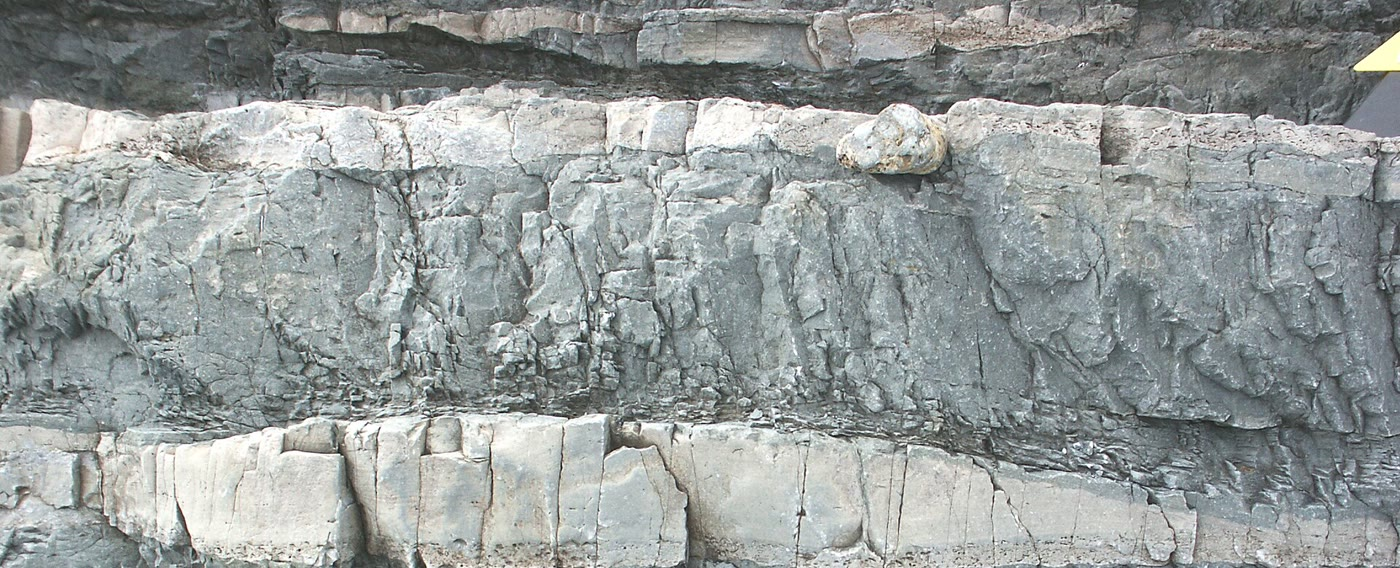
\includegraphics[width=\linewidth]{images/book5/b3-hummocky-cross-stratification.jpg}

{\scriptsize \omterm{def:b3:facies-models:hcs}{Stratification oblique en mamelons} dans la formation d'Arisaig
(Silurien), près d'Arisaig, Nouvelle-Écosse. Photo Michael C. Rygel, CC BY-SA 3.0
(recadrée).}
\end{minipage}
\end{inthefield}
% ledger: photo:b3-hcs

Là où les marées dominent, le faciès change~: les courants de flot et de jusant construisent
des stratifications obliques de sens opposés, des draps de boue se déposent à chaque étale,
et l'épaisseur des ensembles compris entre les draps croît et décroît avec le cycle des marées
de vives-eaux et de mortes-eaux. Les chenaux de marée, les estrans et les crêtes de sable
ont leurs propres modèles, construits de la même manière.

\section{Milieu profond}\label{sec:b3:facies-models:deep}

Un courant de turbidité qui ralentit dépose sa charge selon l'ordre de sédimentation~:
les grains les plus grossiers d'abord, les plus fins en dernier. Un banc de turbidite complet
présente cet ordre sous la forme de cinq divisions.

\begin{definition}[Séquence de Bouma]\label{def:b3:facies-models:bouma}
La \emph{séquence de Bouma}\index{séquence de Bouma} est la succession idéale de
divisions d'un banc de turbidite, de la base au sommet~: Ta, sable massif ou granoclassé sur
une base érosive à marques de courant et d'outil~; Tb, sable à lamination parallèle~; Tc,
sable fin à rides et lamines convolutes~; Td, silt à lamination parallèle~;
Te, boue, en partie issue du courant de turbidité et en partie de la sédimentation lente
entre les écoulements.
\end{definition}

Peu de bancs présentent les cinq divisions~: près de la source, le courant est rapide et laisse
des divisions Ta épaisses, dont les parties supérieures sont érodées par l'écoulement suivant~;
loin de celle-ci, seules arrivent les divisions les plus fines, de Tc à Te. La séquence enregistre
l'affaiblissement d'un écoulement, et le changement des bancs le long de l'éventail enregistre
l'affaiblissement des écoulements avec la distance.

\begin{definition}[Éventail sous-marin]\label{def:b3:facies-models:fan}
Un \emph{éventail sous-marin}\index{eventail sous-marin@éventail sous-marin} est un cône de sédiments au pied
d'un talus continental, alimenté par un canyon~: un éventail supérieur avec un chenal principal
entre des levées, un éventail moyen de chenaux distributaires se terminant par des lobes de sable,
et un éventail inférieur de fines turbidites passant à une boue de plaine abyssale.
\end{definition}

Le long de la marge, les courants profonds entraînés par la circulation océanique remanient
les sédiments fins du talus en contourites, en monticules et en dérives de silt et de boue
bioturbés, qui croissent le long des isobathes plutôt que dans le sens
de la pente.

\begin{omfigure}
\begin{tikzpicture}[font=\scriptsize, x=1cm, y=1cm]
% (a) Bouma log
\begin{scope}
\fill[yellow!45] (0,0) -- (1.6,0) -- (1.6,1.2) -- (0,1.2) -- cycle;
\fill[yellow!35] (0,1.2) rectangle (1.3,1.8);
\fill[yellow!25] (0,1.8) rectangle (1.0,2.4);
\fill[black!12] (0,2.4) rectangle (0.7,2.8);
\fill[black!25] (0,2.8) rectangle (0.4,3.3);
\draw (0,0) -- (1.6,0) -- (1.6,1.2) -- (1.3,1.2) -- (1.3,1.8) -- (1.0,1.8) -- (1.0,2.4) -- (0.7,2.4) -- (0.7,2.8) -- (0.4,2.8) -- (0.4,3.3) -- (0,3.3) -- cycle;
\draw[decorate, decoration={snake, amplitude=0.5mm, segment length=2mm}] (0,0) -- (1.6,0);
\foreach \y in {1.35,1.5,1.65} {\draw[black!60] (0.05,\y) -- (1.25,\y);}
\foreach \x in {0.15,0.45,0.75} {\draw[black!60] (\x,1.95) .. controls (\x+0.08,2.1) .. (\x+0.2,1.95);}
\foreach \y in {2.5,2.6,2.7} {\draw[black!60] (0.05,\y) -- (0.65,\y);}
\foreach \y/\t in {0.6/Ta, 1.5/Tb, 2.1/Tc, 2.6/Td, 3.05/Te} {\node[anchor=west] at (1.9,\y) {\t};}
\node[anchor=west, align=left, font=\tiny] at (2.4,0.6) {sable granoclassé ou massif,\\ base érosive};
\node[anchor=west, font=\tiny] at (2.4,1.5) {lamines parallèles};
\node[anchor=west, font=\tiny] at (2.4,2.1) {rides, lamines convolutes};
\node[anchor=west, font=\tiny] at (2.4,2.6) {silt lité};
\node[anchor=west, font=\tiny] at (2.4,3.05) {boue};
\node[anchor=north] at (1.6,-0.15) {(a) un banc de turbidite};
\end{scope}
% (b) fan plan
\begin{scope}[xshift=8.2cm, yshift=0.2cm]
\fill[black!8] (-1.0,-0.2) rectangle (5.6,3.1);
\fill[yellow!20] (0.3,2.9) .. controls (1.6,2.6) and (4.9,2.0) .. (5.2,0.9) .. controls (4.6,-0.1) and (1.2,0.1) .. (0.3,1.6) -- cycle;
\fill[yellow!45] (1.9,1.9) ellipse (0.55 and 0.3);
\fill[yellow!45] (2.6,1.0) ellipse (0.55 and 0.3);
\fill[yellow!45] (3.4,1.75) ellipse (0.5 and 0.28);
\draw[omDef, line width=1.4pt] (-0.9,3.0) .. controls (-0.3,2.8) and (0.4,2.6) .. (1.0,2.2);
\draw[omDef, line width=0.8pt] (1.0,2.2) -- (1.6,1.95);
\draw[omDef, line width=0.8pt] (1.0,2.2) -- (2.3,1.15);
\draw[omDef, line width=0.8pt] (1.0,2.2) .. controls (2.0,2.4) .. (3.1,1.85);
\node[anchor=south west] at (-0.95,3.0) {canyon};
\node[anchor=east] at (0.55,2.0) {levées latérales};
\node[align=center, font=\tiny] at (2.6,1.0) {lobe};
\node at (4.4,0.7) {éventail inférieur};
\node[black!60] at (4.9,2.85) {plaine abyssale};
\node[anchor=north] at (2.3,-0.25) {(b) un éventail sous-marin en plan};
\end{scope}
\end{tikzpicture}

\par\smallskip{\small (a) La \omterm{def:b3:facies-models:bouma}{séquence de Bouma} d'un banc de turbidite complet,
dessinée comme un log de taille de grain (la largeur indique les grains plus grossiers), avec ses cinq divisions. (b)
Un \omterm{def:b3:facies-models:fan}{éventail sous-marin} en plan~: un canyon alimente un chenal entre levées, qui
se divise en chenaux distributaires se terminant par des lobes sableux~; des turbidites minces
se répandent sur l'éventail inférieur.}\label{fig:b3:facies-models:deep}
\end{omfigure}

\section{Plates-formes carbonatées}\label{sec:b3:facies-models:carbonates}

Le sédiment carbonaté se forme sur place, par l'action d'organismes dans une eau chaude, claire
et peu profonde, et ses faciès suivent le profil de la plate-forme que
l'usine à carbonates construit pour elle-même.

\begin{definition}[Rampe carbonatée et plate-forme à barrière]\label{def:b3:facies-models:ramp}
Une \emph{rampe carbonatée}\index{rampe carbonatée} est une plate-forme dont le fond
s'incline doucement et régulièrement depuis le rivage jusque dans le bassin, sans rupture~:
ses ceintures de faciès, des replats de marée et des sables de plage-barrière jusqu'aux grains de haut-fond,
aux sables bioclastiques et aux boues calcaires du large, sont larges et passent
progressivement les unes aux autres, triées par l'énergie des vagues qui décroît avec la profondeur. Une \emph{plate-forme
à barrière}\index{plate-forme à barrière} est une plate-forme à sommet plat, avec une rupture de pente marquée
à sa marge, où des récifs et des hauts-fonds sableux édifient une barrière qui abrite
un lagon en arrière~; au-delà de la barrière, une pente raide déverse blocs et grains dans le
bassin.
\end{definition}

\begin{omfigure}
\begin{tikzpicture}[font=\scriptsize, x=1cm, y=1cm]
\begin{scope}
\fill[omSea!60] (0,1.6) -- (6.4,1.6) -- (6.4,0.3) -- cycle;
\fill[black!10] (0,1.6) -- (6.4,0.3) -- (6.4,0) -- (0,0) -- cycle;
\draw[thick] (0,1.7) -- (0.3,1.6) -- (6.4,0.3);
\draw[omDef] (0,1.6) -- (6.4,1.6);
\node[anchor=south] at (0.6,1.65) {replat de marée};
\node[rotate=-12, font=\tiny] at (1.5,1.08) {haut-fond};
\node[rotate=-12, font=\tiny] at (3.4,0.66) {sable bioclastique};
\node[rotate=-12, font=\tiny] at (5.3,0.26) {boue calcaire};
\node[anchor=north] at (3.2,-0.1) {(a) rampe~: pente régulière};
\end{scope}
\begin{scope}[xshift=7.2cm]
\fill[omSea!60] (0,1.6) -- (6.4,1.6) -- (6.4,0.2) -- (4.4,0.3) -- (3.6,1.55) -- (3.2,1.6) -- (0.3,1.6) -- cycle;
\fill[omSea!60] (0.3,1.6) -- (3.2,1.6) -- (3.0,1.35) -- (0.6,1.35) -- cycle;
\fill[black!10] (0,1.7) -- (0.3,1.6) -- (0.6,1.35) -- (3.0,1.35) -- (3.2,1.6) -- (3.6,1.55) -- (4.4,0.3) -- (6.4,0.2) -- (6.4,0) -- (0,0) -- cycle;
\draw[thick] (0,1.7) -- (0.3,1.6) -- (0.6,1.35) -- (3.0,1.35) -- (3.2,1.6) -- (3.6,1.55) -- (4.4,0.3) -- (6.4,0.2);
\fill[orange!50] (3.05,1.4) -- (3.2,1.6) -- (3.55,1.56) -- (3.6,1.4) -- cycle;
\draw[omDef] (0,1.6) -- (6.4,1.6);
\node at (1.8,1.12) {lagon};
\node[anchor=south] at (3.35,1.65) {barrière récifale};
\node[anchor=west] at (4.2,0.95) {pente raide};
\node at (5.5,0.6) {bassin};
\node[anchor=north] at (3.2,-0.1) {(b) plate-forme à barrière};
\end{scope}
\end{tikzpicture}

\par\smallskip{\small Profils de plates-formes carbonatées (schématiques, échelle verticale
fortement exagérée). (a) Une rampe~: ceintures triées par l'énergie des vagues le long d'une pente
régulière. (b) Une \omterm{def:b3:facies-models:ramp}{plate-forme à barrière}~: un récif et une barrière de hauts-fonds à la rupture de pente
abrite un lagon de boue calcaire~; la pente au-delà reçoit blocs et grains
issus de la barrière.}\label{fig:b3:facies-models:platforms}
\end{omfigure}

Sur le sommet plat d'une plate-forme, une faible hausse du niveau marin relatif inonde les
replats de marée, et l'usine, qui travaille le plus vite dans l'eau la moins profonde, comble
l'espace jusqu'au niveau de la mer en peu de temps. Il en résulte un empilement de cycles
péritidaux d'un mètre ou de quelques mètres d'épaisseur, chacun une \omterm{def:b3:sequence-stratigraphy:parasequence}{paraséquence} à tendance
régressive, allant de boues subtidales à un replat de marée portant des fentes de dessiccation ou
des tapis microbiens, coiffée par la \omterm{def:b3:sequence-stratigraphy:parasequence}{surface d'inondation} suivante.

\section{Carottes et diagraphies}\label{sec:b3:facies-models:logs}

La majeure partie des roches sous les bassins sédimentaires est connue grâce aux forages. Quelques
forages sont carottés, et leurs carottes sont décrites banc par banc, comme une falaise~; presque
tous sont diagraphiés.

\begin{definition}[Diagraphies]\label{def:b3:facies-models:wireline}
Une \emph{diagraphie}\index{diagraphie} est un enregistrement continu d'une
propriété physique des roches en fonction de la profondeur, mesurée par une sonde descendue
au bout d'un câble dans un forage. La \emph{diagraphie gamma}\index{diagraphie gamma}
enregistre la radioactivité gamma naturelle de la roche, en unités API~: forte dans les argiles,
dont les minéraux retiennent potassium, thorium et uranium, faible dans le sable de quartz
propre et dans le calcaire. La \emph{diagraphie de densité}\index{diagraphie de densité}
enregistre la masse volumique apparente d'après la diffusion des rayons gamma émis par une
source placée sur la sonde. La \emph{diagraphie sonique}\index{diagraphie sonique} enregistre le
temps de transit par intervalle d'une onde de compression, en microsecondes par pied. La
\emph{diagraphie neutron}\index{diagraphie neutron} enregistre le ralentissement des neutrons par
l'hydrogène, et donc l'eau retenue dans les pores et dans les argiles.
\end{definition}
% ledger: keys:gamma, keys:density-porosity, keys:sonic

L'unité API de rayonnement gamma est définie dans une fosse d'étalonnage~: un deux-centième de
la différence entre une zone de radioactivité négligeable et une zone contenant
les radioisotopes d'une argile moyenne à environ deux fois sa concentration. Le charbon,
le calcaire et la dolomie sont généralement moins radioactifs que les argiles~; le grès
quartzeux est faible, une arkose riche en feldspath potassique l'est davantage~; toute roche peut être
rendue radioactive par l'uranium apporté par les eaux souterraines.
% ledger: keys:gamma

\begin{proposition}[Porosité à partir de la masse volumique et du temps de transit]\label{prop:b3:facies-models:porosity}
Une roche de porosité $\phi$, dont les grains ont une masse volumique $\rho_{\mathrm{ma}}$ et
des pores remplis d'un fluide de masse volumique $\rho_f$, a pour masse volumique globale
$\rho_b = (1 - \phi)\rho_{\mathrm{ma}} + \phi\rho_f$, de sorte que
\[
\phi = \frac{\rho_{\mathrm{ma}} - \rho_b}{\rho_{\mathrm{ma}} - \rho_f}.
\]
Si une onde de compression traverse les grains et le fluide en série, sur des
longueurs proportionnelles à $1 - \phi$ et $\phi$, son temps de transit est
$\Delta t = (1 - \phi)\Delta t_{\mathrm{ma}} + \phi\Delta t_f$ (la
équation de la moyenne temporelle), et $\phi = (\Delta t - \Delta
t_{\mathrm{ma}})/(\Delta t_f - \Delta t_{\mathrm{ma}})$.
\end{proposition}

\begin{proof}
Un volume unitaire de roche contient un volume $1 - \phi$ de grains et $\phi$ de
fluide~; sa masse vaut $(1 - \phi)\rho_{\mathrm{ma}} + \phi\rho_f$, équation dont on tire
$\phi$. Pour l'onde, un trajet de longueur unitaire traverse $1 - \phi$ de grains
et $\phi$ de fluide, et les temps s'ajoutent.
\end{proof}

Les masses volumiques des grains valent \qty{2.65}{g/cm^3} pour le quartz et \qty{2.71}{g/cm^3} pour
le calcaire~; l'eau interstitielle vaut \qty{1.0}{g/cm^3} lorsqu'elle est douce et
jusqu'à \qty{1.1}{g/cm^3} en saumure. Les temps de transit vont de 42 à
\qty{48}{\micro\second/ft} dans la dolomie, de 48 à 53 dans le calcaire, 53 pour un
grès consolidé, et 189 dans la saumure. L'équation de la masse volumique est exacte pour
une matrice connue~; l'équation de la moyenne temporelle est une règle empirique qui fonctionne
au mieux dans les roches consolidées à pores intergranulaires. Les argiles mettent en défaut les deux~:
elles ont leurs propres masses volumiques et retiennent de l'eau liée.
% ledger: keys:density-porosity, keys:sonic

\begin{definition}[Rapport net sur brut]\label{def:b3:facies-models:ntg}
Le \emph{rapport net sur brut}\index{rapport net sur brut} d'un intervalle est l'épaisseur de
sa roche de qualité réservoir, généralement le sable identifié sur la \omterm{def:b3:facies-models:wireline}{diagraphie gamma}
sous un seuil de coupure, divisée par l'épaisseur totale de l'intervalle.
\end{definition}

La forme de la courbe gamma à travers un corps sableux est un outil de faciès.
Une \emph{cloche}, propre à la base et plus argileuse vers le haut, correspond à une \omterm{def:b3:facies-models:association}{succession
granodécroissante}, comme dans une \omterm{def:b3:facies-models:rivers}{barre de méandre} ou un remplissage de chenal~; un \emph{entonnoir}, argileux à
la base et propre au sommet, correspond à une \omterm{def:b3:facies-models:association}{succession granocroissante}, comme dans un
\omterm{def:b3:facies-models:shoreface}{avant-côte} progradant ou un front deltaïque~; un \emph{cylindre}, propre sur toute sa hauteur,
avec des limites nettes, correspond à un sable de \omterm{def:b3:facies-models:rivers}{rivière en tresses} empilé, à une dune éolienne ou à un
haut-fond carbonaté. Ces formes sont des indices, non des preuves~: une carotte, ou du moins les
\omterm{def:b3:facies-models:wireline}{diagraphies} voisines, doit les confirmer.

\begin{omfigure}
\begin{tikzpicture}
\begin{groupplot}[group style={group size=3 by 1, horizontal sep=0.2cm,
    y descriptions at=edge left},
  omrecord, y dir=reverse, ymin=700, ymax=1200, width=0.28\linewidth,
  height=0.62\linewidth, ytick={700,800,900,1000,1100,1200},
  tick label style={font=\scriptsize}, label style={font=\small},
  xlabel style={font=\small}]
\nextgroupplot[xlabel={GR (API)}, ylabel={profondeur (m)}, xmin=0, xmax=150,
  xtick={0,50,100,150}]
\addplot[black!60, densely dashed, forget plot] coordinates {(60,1046) (60,1166)};
% computed in figdata/bachelor-3/well_logs.py
\addplot[omDef, thin] table[x=gr, y=depth] {figdata/out/bachelor-3-well_logs-logs.dat};
\node[font=\scriptsize, anchor=west] at (axis cs:2,730) {craie};
\node[font=\scriptsize, anchor=west] at (axis cs:2,816) {argile};
\node[font=\scriptsize, anchor=west] at (axis cs:28,956) {calcaire};
\node[font=\scriptsize, anchor=west] at (axis cs:28,1030) {grès};
\node[font=\scriptsize, anchor=west] at (axis cs:2,1185) {schiste};
\nextgroupplot[xlabel={$\rho_b$ (\unit{g/cm^3})}, xmin=1.9, xmax=2.9,
  xtick={2.0,2.4,2.8}, xticklabels={2.0,2.4,2.8}]
\addplot[red!70!black, thin] table[x=rhob, y=depth] {figdata/out/bachelor-3-well_logs-logs.dat};
\nextgroupplot[xlabel={$\Delta t$ (\unit{\micro\second/ft})}, xmin=40, xmax=140,
  x dir=reverse, xtick={40,80,120}]
\addplot[green!40!black, thin] table[x=dt, y=depth] {figdata/out/bachelor-3-well_logs-logs.dat};
\end{groupplot}
\begin{axis}[at={(group c3r1.south east)}, xshift=1.35cm, anchor=south west,
  omrecord, y dir=reverse, ymin=1040, ymax=1172, width=0.28\linewidth,
  height=0.62\linewidth, xmin=0, xmax=120, xtick={0,60,120},
  ytick={1040,1060,1080,1100,1120,1140,1160}, ylabel={profondeur (m)},
  xlabel={GR (API), grès}, tick label style={font=\scriptsize},
  label style={font=\small}]
\addplot[black!60, densely dashed, forget plot] coordinates {(60,1046) (60,1166)};
\addplot[omDef, semithick] table[x=gr, y=depth] {figdata/out/bachelor-3-well_logs-sand.dat};
\end{axis}
\end{tikzpicture}

\par\smallskip{\small \omterm{def:b3:facies-models:wireline}{Diagraphies} synthétiques du puits Varden-2, de \qty{700}{m}
jusqu'au socle~: rayonnement gamma (la ligne en tirets marque le seuil de coupure du sable, soit
\qty{60}{API} dans le grès), masse volumique globale et temps de transit sonique (temps
croissant vers la gauche, comme on trace les \omterm{def:b3:facies-models:wireline}{diagraphies})~; à droite, le rayonnement gamma du
grès agrandi. La craie se densifie avec la profondeur~;
l'argile apparaît chaude, lente et de masse volumique intermédiaire~; le calcaire est froid,
dense et rapide~; le grès est un empilement de remplissages de chenaux, chacun ayant une base propre
passant vers le haut à de la boue~: formes en cloche.}\label{fig:b3:facies-models:logs}
\end{omfigure}
% ledger: keys:gamma, keys:density-porosity, keys:sonic

\begin{inthelab}[Description d'une carotte]
\begin{minipage}[t]{0.5\linewidth}\vspace{0pt}
Dans un entrepôt de carottes, les carottes d'un puits sont disposées en caisses, fendues
sur leur longueur, dans l'ordre de leur profondeur. Un sédimentologue décrit la carotte
banc par banc sur une fiche de description~: taille des grains à la loupe et à l'aide d'une
charte de comparaison, structures, contacts, fossiles, traces de terriers et de racines, couleur de la boue.
La description est ensuite placée à côté des \omterm{def:b3:facies-models:wireline}{diagraphies} de
mêmes profondeurs, ce qui permet d'étalonner la forme des \omterm{def:b3:facies-models:wireline}{diagraphies} par rapport à la roche et de lire les
puits voisins non carottés.
\end{minipage}\hfill
\begin{minipage}[t]{0.46\linewidth}\vspace{0pt}
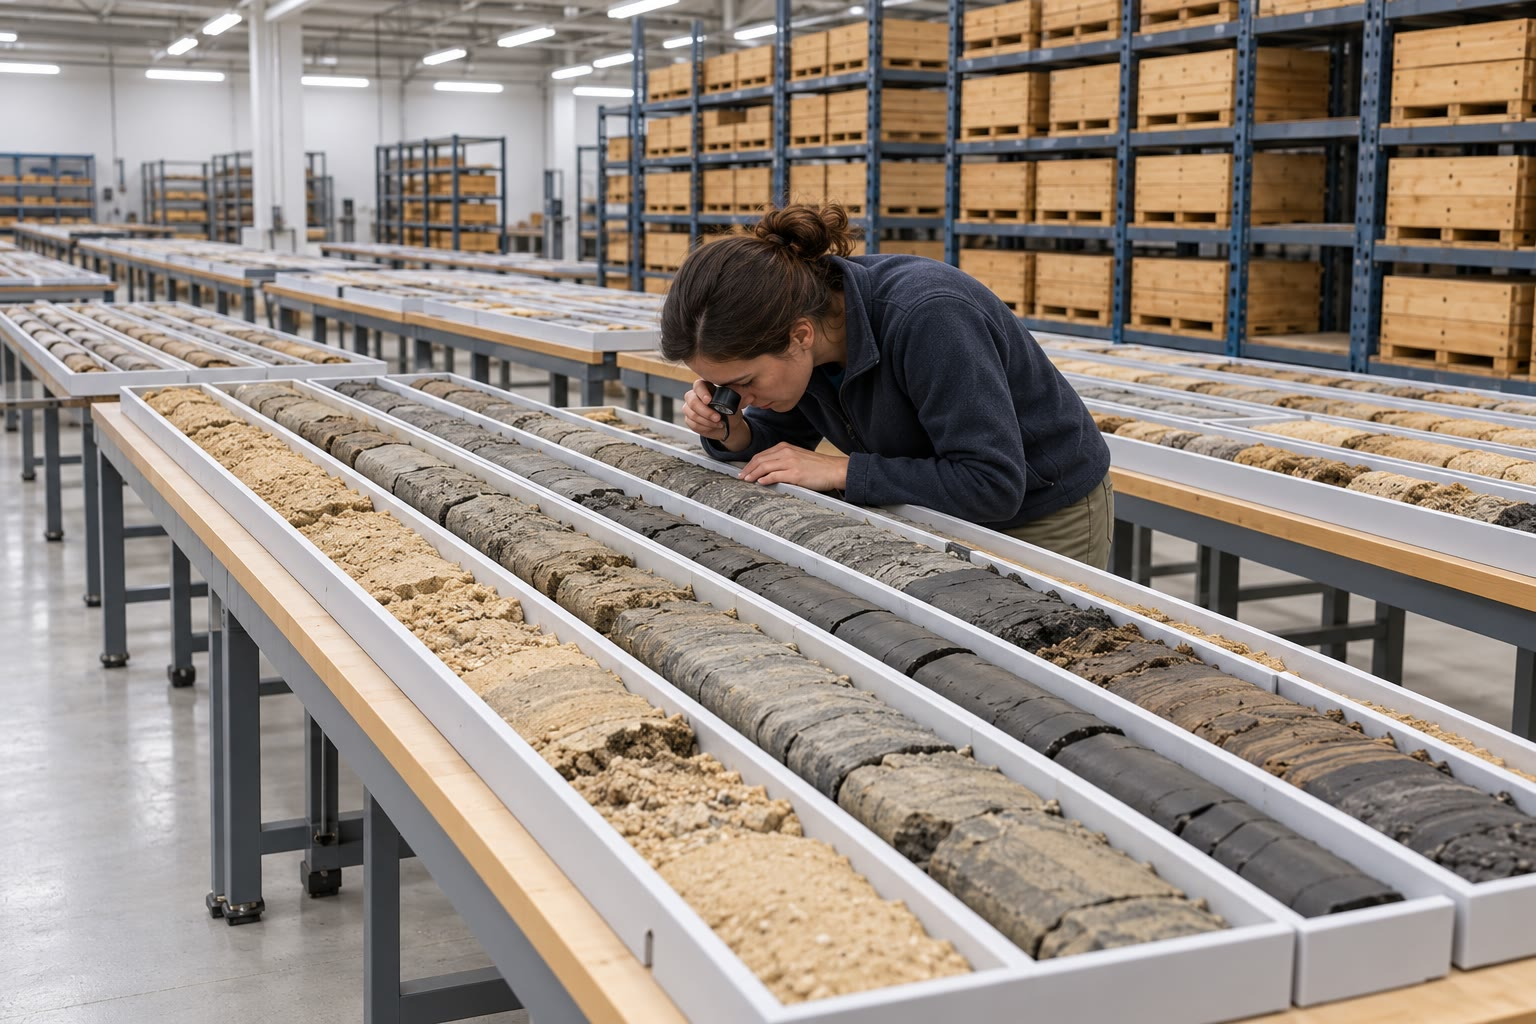
\includegraphics[width=\linewidth]{images/book5/ai/b3-core-store.jpg}

{\scriptsize Un entrepôt de carottes~: carottes de sable et de boue fendues en caisses, un géologue
à la loupe. Illustration générée par IA.}
\end{minipage}
\end{inthelab}

\section{Exercices}

\begin{exercise}[$\star$]\label{exo:b3:facies-models:1}
Une carotte présente, de la base vers le haut~: boue du large, boue et sable fin interstratifiés,
sable d'\omterm{def:b3:facies-models:shoreface}{avant-côte}, sable de plage, puis charbon à racines. En utilisant la loi de Walther, donner
l'ordre des milieux le long de la côte à cette époque et le sens
dans lequel le rivage s'est déplacé. Qu'aurait laissé une transgression~?
\end{exercise}

\begin{exercise}[$\star$]\label{exo:b3:facies-models:2}
Trois corps sableux présentent des formes de rayonnement gamma~: (a) une cloche de \qty{8}{m} d'épaisseur
à base nette~; (b) un entonnoir de \qty{20}{m} d'épaisseur~; (c) un cylindre de \qty{30}{m}
d'épaisseur à sommet et base nets. Proposer un milieu pour chacun, et
l'observation dans une carotte qui le confirmerait.
\end{exercise}

\begin{exercise}[$\star$]\label{exo:b3:facies-models:3}
Un grès présente $\rho_b = \qty{2.40}{g/cm^3}$. Calculer sa porosité avec une
matrice de quartz et d'eau douce, puis avec une saumure de \qty{1.1}{g/cm^3}.
\end{exercise}
% ledger: keys:density-porosity

\begin{exercise}[$\star$]\label{exo:b3:facies-models:4}
Ondes de longueur d'onde modale \qty{75}{m} et \qty{110}{m} (les mers abritée
et ouverte de l'étude par bouée). Estimer la profondeur à laquelle chacune conserve
\qty{4}{\percent} de son mouvement de surface, et la fraction restante à une
profondeur de \qty{20}{m}.
\end{exercise}
% ledger: losspeters10:wavebase

\begin{exercise}[$\star\star$]\label{exo:b3:facies-models:5}
Un calcaire présente $\Delta t = \qty{60}{\micro\second/ft}$. Calculer sa
porosité avec l'équation de moyenne temporelle pour une matrice de 47.6 et de
\qty{52.6}{\micro\second/ft} et une saumure à \qty{189}{\micro\second/ft}.
Qu'enseigne la différence~?
\end{exercise}
% ledger: keys:sonic

\begin{exercise}[$\star\star$]\label{exo:b3:facies-models:6}
Un intervalle de \qty{40}{m} renferme des bancs de sable de 6.0, 3.5, 8.0 et \qty{2.5}{m}
au-dessous du seuil, le reste étant de la boue. Calculer son \omterm{def:b3:facies-models:ntg}{rapport net sur brut}. Avec une
porosité de \qty{22}{\percent} dans le sable, quel volume de pores contient
un kilomètre carré de cet intervalle~?
\end{exercise}

\begin{exercise}[$\star\star$]\label{exo:b3:facies-models:7}
Un banc turbiditique près de l'embouchure d'un canyon est formé de \qty{1.2}{m} de sable massif
(Ta) érodé au sommet par le banc suivant~; à \qty{30}{km} en aval de l'éventail, un banc
du même écoulement se compose de \qty{8}{cm} de sable fin et de silt à rides laminées, sous
\qty{3}{cm} de boue. Nommer les divisions de chacun et expliquer le changement.
\end{exercise}

\begin{exercise}[$\star\star$]\label{exo:b3:facies-models:8}
Une \omterm{def:b3:facies-models:association}{succession granodécroissante} de \qty{9}{m} d'épaisseur présente une base nette à galets,
du sable à stratification oblique, du sable fin à rides et de la boue à racines. L'interpréter, et
estimer la profondeur du chenal qui l'a construite. La loi de Walther peut-elle
s'appliquer au travers de sa base~? Pourquoi~?
\end{exercise}

\begin{exercise}[$\star\star$]\label{exo:b3:facies-models:9}
Un plancher de plate-forme descend de \qty{60}{m} sur \qty{40}{km}~; une autre conserve
une profondeur de \qty{5}{m} sur \qty{30}{km}, puis descend de \qty{300}{m} sur
\qty{1.5}{km}. Calculer les deux gradients, nommer chaque plate-forme et le faciès
attendu au bord de la seconde.
\end{exercise}

\begin{exercise}[$\star\star\star$]\label{exo:b3:facies-models:10}
Un rivage progradant à une vitesse $v$ tandis que le niveau marin relatif monte à un taux
$A$, et sa ceinture d'\omterm{def:b3:facies-models:shoreface}{avant-côte} a une largeur $w$. Montrer que le sable d'\omterm{def:b3:facies-models:shoreface}{avant-côte} dans la
succession verticale a pour épaisseur $h = wA/v$. La calculer pour $w = \qty{2}{km}$,
$A = \qty{0.2}{m/ka}$ et $v = \qty{20}{m/ka}$, et dire ce qui se passe lorsque
$A = 0$. Comparer avec la proposition sur la \omterm{def:b3:sequence-stratigraphy:trajectory}{trajectoire du rivage}
figurant au chapitre~\ref{ch:b3:sequence-stratigraphy}.
\end{exercise}

\begin{exercise}[$\star\star\star$]\label{exo:b3:facies-models:11}
Un grès présente $\rho_b = \qty{2.30}{g/cm^3}$ et $\Delta t =
\qty{86}{\micro\second/ft}$. Calculer sa porosité à partir de chaque \omterm{def:b3:facies-models:wireline}{diagraphie}, avec une
matrice de grès quartzeux (2.65, \qty{52.6}{\micro\second/ft}) et une saumure (1.0 pour la
masse volumique, \qty{189}{\micro\second/ft}). Si la porosité sonique est juste, quelle
masse volumique des grains implique la \omterm{def:b3:facies-models:wireline}{diagraphie de densité}, et quel peut être le ciment~?
\end{exercise}
% ledger: keys:density-porosity, keys:sonic

\begin{exercise}[$\star\star\star$]\label{exo:b3:facies-models:12}
Dans une carotte, de la boue marine noire repose directement sur un charbon à racines, avec une
fine couche de débris coquilliers au contact. Expliquer pourquoi la loi de Walther ne
s'applique pas au travers de celle-ci, quelle surface c'est, et quelle part de la
succession côtière peut manquer si les vagues ont érodé le plancher jusqu'à une
\omterm{def:b3:facies-models:shoreface}{limite d'action des vagues de beau temps} d'environ \qty{10}{m} lorsque le rivage est passé.
\end{exercise}

\section{Problème~: Varden-2, un puits à travers la couverture}

\begin{problem}[{Problème du week-end --- les diagraphies, la porosité, les faciès et le
sable net d'un puits fictif du synclinal de Varden}]
\label{pb:b3:facies-models:1}
Le puits Varden-2 est foré dans le synclinal des collines de Varden, aux
coordonnées (7500, 7000) de la grille régionale, depuis une altitude du sol de
\qty{441.0}{m}, jusqu'à une profondeur totale de \qty{1200}{m}. Ses \omterm{def:b3:facies-models:wireline}{diagraphies} sont tracées dans la
figure de la dernière section. Utiliser des masses volumiques des grains de 2.65 (quartz) et
\qty{2.71}{g/cm^3} (calcite), une eau interstitielle de \qty{1.0}{g/cm^3}, des temps de
transit de matrice de 52.6 (grès) et \qty{47.6}{\micro\second/ft}
(calcaire), et \qty{189}{\micro\second/ft} pour l'eau.

\medskip\noindent\textbf{Partie I --- Lecture des diagraphies.}
\begin{enumerate}
\item Le rayonnement gamma bondit de 12 à \qty{110}{API} à \qty{766}{m}, puis
  chute à 18 à \qty{866}{m}, devient irrégulier à partir de \qty{1046}{m} et stable à
  \qty{85}{API} à partir de \qty{1166}{m}. Nommer les unités rencontrées, à l'aide de leurs \omterm{def:b3:facies-models:wireline}{diagraphies}.
\item Calculer l'épaisseur de chaque unité de la couverture et l'altitude de
  la base de la couverture.
\item La craie présente \qty{2.03}{g/cm^3} près de la surface et
  \qty{2.36}{g/cm^3} à \qty{750}{m}. Calculer sa porosité aux deux profondeurs.
  Que devient la craie avec la profondeur~?
\item Pourquoi ne peut-on pas attribuer une porosité à l'argilite à partir de sa masse volumique~?
\item Le schiste présente \qty{2.75}{g/cm^3} et \qty{50}{\micro\second/ft}.
  Que révèle le socle rapide, dense et sans porosité au foreur~?
\end{enumerate}

\medskip\noindent\textbf{Partie II --- Porosité.}
\begin{enumerate}[resume]
\item Le calcaire présente \qty{2.573}{g/cm^3}~: calculer sa porosité de densité.
\item Il présente \qty{58.9}{\micro\second/ft}~: calculer sa porosité sonique et
  la comparer.
\item Le sable propre des remplissages de chenal présente \qty{2.32}{g/cm^3}~: calculer
  sa porosité.
\item Vérifier-la avec son temps de transit, \qty{79.9}{\micro\second/ft}.
\item Si l'eau interstitielle était une saumure de \qty{1.1}{g/cm^3}, de combien changerait
  la porosité de densité du sable~?
\item Quelle unité ferait le meilleur aquifère ou réservoir, et laquelle
  constitue la roche couverture qui la surmonte~?
\end{enumerate}

\medskip\noindent\textbf{Partie III --- Faciès.} Une carotte prélevée de 1108 à
\qty{1124}{m} montre, de la base vers le haut~: une surface érodée à galets argileux et
graviers~; \qty{10.4}{m} de sable moyen à stratification oblique~; \qty{3.2}{m} de sable fin
à ondulations passant à des silts~; \qty{2.4}{m} de boue brun-rouge à traces de racines.
\begin{enumerate}[resume]
\item Tracer la forme du rayonnement gamma attendue au droit de l'intervalle carotté.
\item Nommer la succession et le milieu de dépôt de chaque partie.
\item À l'aide de la loi de Walther, décrire les milieux qui se succèdent latéralement.
\item Estimer la profondeur du chenal.
\item Le grès renferme onze unités de ce type, chacune reposant sur une base nette. Que
  révèle l'empilement sur la rivière et sa plaine~?
\item La loi de Walther peut-elle servir à passer d'une unité à la suivante~? Pourquoi~?
\end{enumerate}

\medskip\noindent\textbf{Partie IV --- Sable net.} Les onze remplissages de chenal,
à partir de la base du grès, mesurent 14, 9, 12, 7, 16, 10, 13, 8, 11, 12 et
\qty{8}{m} d'épaisseur. Chacun débute par un sable propre (\qty{30}{API}) sur une
fraction de son épaisseur de 0.60, 0.45, 0.55, 0.30, 0.65, 0.40, 0.55, 0.35, 0.50,
0.45 et 0.30, puis s'affine vers le haut sur une fraction de 0.25, 0.30, 0.25, 0.40,
0.20, 0.30, 0.25, 0.35, 0.25, 0.30 et 0.35, le rayonnement gamma croissant linéairement jusqu'à
\qty{105}{API}, et se termine par de la boue.
\begin{enumerate}[resume]
\item Quelle fraction de chaque intervalle granodécroissant se situe sous le
  seuil de \qty{60}{API}~?
\item Calculer le sable net de l'unité la plus basse et de la plus épaisse.
\item Calculer le total de sable propre et le total des intervalles granodécroissants du
  grès.
\item Calculer son \omterm{def:b3:facies-models:ntg}{rapport net sur brut}.
\item Comment varierait le sable net avec un seuil de 45 ou de
  \qty{75}{API}~?
\item Avec la porosité du sable de la question~8, calculer le volume poreux du
  sable net sous un kilomètre carré.
\item Donner l'épaisseur de sable net du grès triasique de Varden-2.
\end{enumerate}
\end{problem}
% ledger: keys:density-porosity, keys:sonic, keys:gamma
